\documentclass[10pt,a4paper]{article}
\usepackage[utf8]{inputenc}
\usepackage[T1]{fontenc}
\usepackage{amsmath}
\usepackage{amsfonts}
\usepackage{amssymb}
\usepackage{graphicx}
\usepackage{physics}
\usepackage{cite}
\usepackage{caption}
\usepackage{subcaption}
\usepackage{hyperref}
\usepackage{comment}

\linespread{1.2}
\usepackage[a4paper,top=3cm,bottom=3cm,left=3cm,right=3cm]{geometry}

\title{Ergotropy close to a Quantum Phase Transition }
\author{}



\begin{document}
	\maketitle
	\section{Goal}
	 Ergotropy \cite{allahverdyan2004maximal} is the maximum work that can be extracted from a system using only unitary operations:\\
	 \begin{equation}\label{eq:ergotropy}
	 W=\max_U [ Tr(\rho H)- Tr(U\rho U^{\dagger} H) ]
	 \end{equation}
	 It can be shown \cite{allahverdyan2004maximal} that:
	
	\begin{equation}\label{eq:ergotropy2}
	W= Tr(\rho H)- Tr(\rho_{pass} H) =E(\rho)-E(\rho_{pass})
	\end{equation}
	with:
		\begin{equation}\label{eq:ergotropy3}
	\rho_{pass}=\sum_{j} r_{j}\left|\varepsilon_{j}\right\rangle\left\langle\varepsilon_{j}\right|
	\end{equation}
	$ \lbrace r_j \rbrace$=eigenvalues of $\rho$ sorted in descending order \\
	$ \lbrace \epsilon_j \rbrace$= eigenvalues of H sorted in ascending order \\
	Intuitively, the "most probable" states are the "less energetic" one.\\
	We want to study the behaviour of Ergotropy when the system is close to a Quantum Phase Transition.
	
	\section{Ising Model}
	
	The simplest model that undergoes a Quantum Phase Transition is the Ising Model.
	The model is defined by the lattice Hamiltonian (we use the convention of \cite{latorre2003ground} pag.9, the Ising Model is the XY model with $\gamma=1$):
	\begin{equation}\label{eq:hamilt}
	H=-\frac{1}{2} \sum_{l=-\frac{N-1}{2}}^{\frac{N-1}{2}}\left(\sigma_{l}^{x} \sigma_{l+1}^{x}+\lambda\sigma_{l}^{z}\right)
	\end{equation}
	
	With $\lambda \in \real$. For now we limit ourselves to a 1D spin chain with periodic boundaries.\\ 
	It's important to notice some points:
	\begin{enumerate}
		\item The system has a symmetry for $\lambda \rightarrow -\lambda$ followed by a z-inversion, so we will study it only for $\lambda>0$
		\item For $\lambda \rightarrow \infty$ the ground state is the state $\ket{\uparrow\uparrow\uparrow \dots} $
		\item For $\lambda=0$ the ground states are : $\ket{\rightarrow\rightarrow\rightarrow \dots} \quad \text{and} \quad \ket{\leftarrow\leftarrow\leftarrow\dots} $ 
		\item Imposing periodic boundary conditions (the last element of the chain is connected to the first) the chain is translationally invariant so we can choose freely the subsystem to study, also for $N\rightarrow\infty$ the boundary conditions become irrelevant.
	\end{enumerate}
	This model has one quantum critical point: $\lambda=1$ \cite{sachdev_2011} this can be seen for example studying the gap between the ground and the first excited state:
	Fig \ref{fig:energap} is obtained using the Lanczos method \cite{Jaegon_2007}, for $N\rightarrow\infty$ the transition between the gapped and gapless fase becomes sharper, since we are at $T=0$, this is  a QPT.
	

	\begin{figure}[h]
		\centering
		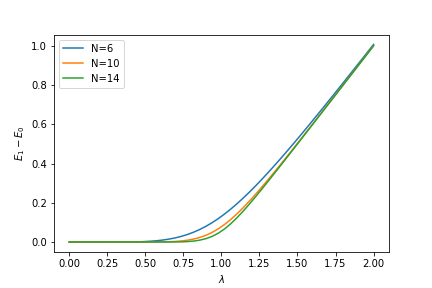
\includegraphics[width=0.7\linewidth]{scalinggap}
		\caption{Energy gap close to the critical point for different lengths, exact diagonalization}
		\label{fig:energap}
	\end{figure}
	
	\subsection{Numerical Ergotropy}\label{sec:numergo}
	
	Using the Lanczos algorithm \cite{Jaegon_2007} (specifically the ARPACK library \cite{arpack})    we exactly diagonalize the Ising Model.\\ With the ground state of the whole chain we can obtain the L-site density matrix and calculate the Ergotropy ( eq.\ref{eq:ergotropy2} ) following these steps:
	\begin{enumerate}
		\item Diagonalize the whole N-sites Hamiltonian and obtain the ground state $\ket{ \psi_g}$
		\item Calculate the L-site reduced density matrix tracing out the remaining N-L sites: $\rho_L=Tr_{N-L}(\ket{ \psi_g}\bra{\psi_g}$) 
		\item Construct the L-site Hamiltonian: 	$H_L=-\frac{1}{2}\sum_{j=0}^{L-1}\left(\sigma_{j}^{x} \sigma_{j+1}^{x}+\lambda\sigma_{j}^{z}\right)$
		\item Build the passive state $\rho^{pass}_L$ \ref{eq:ergotropy3}
		\item Calculate the Ergotropy as the difference $E(\rho_L) - E(\rho^{pass}_L)$ \ref{eq:ergotropy2} 
	\end{enumerate}
	For 2 sites we obtain fig.\ref{fig:calcolilanczos2}  and for 3 sites fig. \ref{fig:calcolilanczos3}
	
	
	
	\begin{figure}[b]
		\centering
		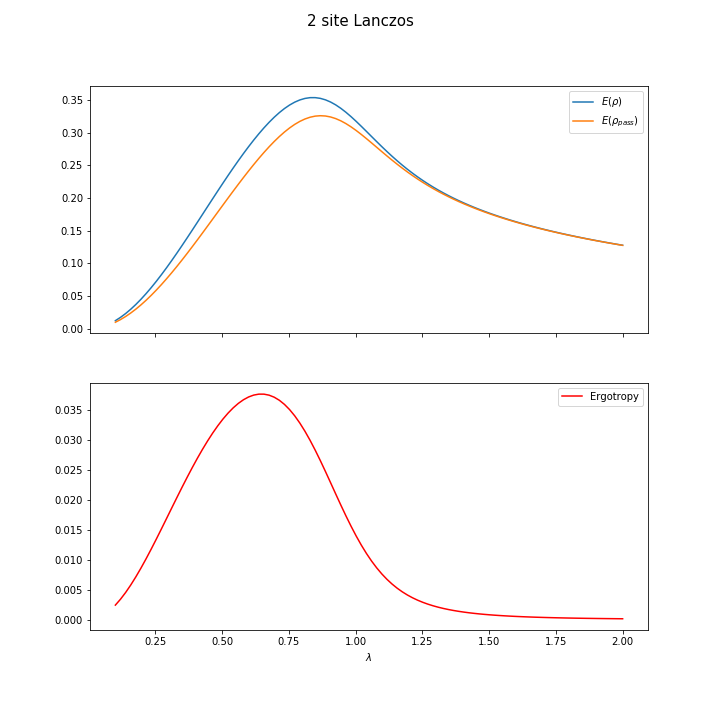
\includegraphics[width=\linewidth]{calcoli_lanczos_2}
		\caption{Results for a N=10 chain,	the energy is rescaled so that it is always positive.}
		\label{fig:calcolilanczos2}
	\end{figure}
	\begin{figure}[b]
		\centering
		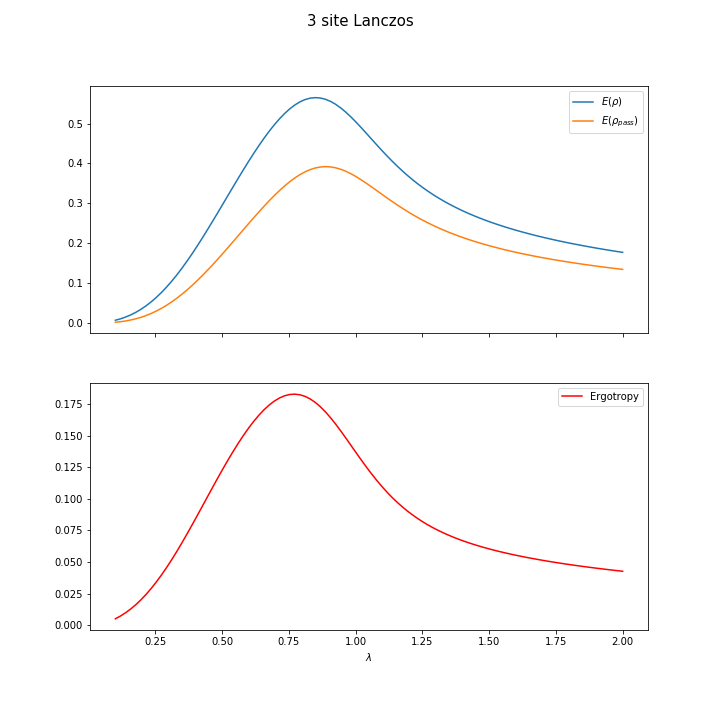
\includegraphics[width=\linewidth]{calcoli_lanczos_3}
		\caption{Results for a N=10 chain,	the energy is rescaled so that it is always positive.}
		\label{fig:calcolilanczos3}
	\end{figure}
	
	\subsection{Analytical Ergotropy}\label{sec:analerg}
	We want to calculate the ergotropy without the need to diagonalize all the system numerically like in sec. \ref{sec:numergo} .\\	
	Looking at eq. \ref{eq:ergotropy2} - \ref{eq:ergotropy3}, to do this we need to find the reduced density matrix and the reduced Hamiltonian for a sub-chain of L sites.\\	
	As we have seen  in sec. \ref{sec:numergo} the Hamiltonian \ref{eq:hamilt} is easy to restrict to L sites, the difficult part is to derive analytically the L-site reduced density matrix.	\\
	\newline
	To get the reduced density matrix we will follow the road map described in [\cite{latorre2003ground} pag.9]:
	\begin{enumerate}
		\item Transform the Hamiltonian using Majorana operators
		\item Write the correlation matrix for the new operators on the ground state of the whole chain
		\item Restrict the correlation matrix to the subsystem of interest
		\item Expand the reduced density matrix in the Pauli basis
		\item Find the density matrix expectation values on the ground state using Wick's theorem 
	\end{enumerate}
In the following calculation we will follow closely the notation in \cite{latorre2003ground}.\\
The non-local transformation:
	\begin{equation}\label{majorana}
	\check{a}_{2 l-1} \equiv\left(\prod_{m<l} \sigma_{m}^{z}\right) \sigma_{l}^{x} ; \quad
	\check{a}_{2 l} \equiv\left(\prod_{m<l} \sigma_{m}^{z}\right) \sigma_{l}^{y}
	\end{equation}
	\begin{equation}\label{eq:anticomm}
	\check{a}_{m}^{\dagger}=\check{a}_{m}, \quad\left\{\check{a}_{m}, \check{a}_{n}\right\}=2 \delta_{m n}\end{equation}
	defines 2N Majorana operators (2 for every site: "even" and "odd") and maps the Hamiltonian \ref{eq:hamilt} to :
	\begin{equation}\label{eq:hamiltwitha}
	H =\frac{i}{2} \sum_{l=-\frac{N-1}{2}}^{\frac{N-1}{2}} \check{a}_{2 l} \check{a}_{2 l+1}  
	+ \lambda \check{a}_{2 l-1} \check{a}_{2 l}
	\end{equation}
	From here we can derive the correlation matrix for the Majorana operators on the ground state of the whole chain (the details of the calculation are shown in \ref{appendixcalculation}):
	\begin{equation}\label{eq:corrmatr1}
	\left\langle\check{a}_{m} \check{a}_{n}\right\rangle=\delta_{m n}+i\left(\Gamma^{A}\right)_{m n}, 
	\end{equation}
	
	\begin{equation}\label{eq:corrmatr2}
	\Gamma^{A}=\left[\begin{array}{cccc}
	\Pi_{0} & \Pi_{1} & \cdots & \Pi_{N-1} \\
	-\Pi_{1}^T & \Pi_{0} & & \vdots \\
	\vdots & & \ddots & \vdots \\
	-\Pi_{N-1}^T & \cdots & \cdots & \Pi_{0}
	\end{array}\right]\end{equation}

	\begin{equation}\label{eq:corrmatr3}
	\Pi_{l}=\left[\begin{array}{cc}
	0 & g_{l} \\
	-g_{-l} & 0
	\end{array}\right] 
	 \quad g_{l}=\frac{1}{2 \pi} \int_{0}^{2 \pi} d \phi e^{-i l \phi} \frac{\lambda-\cos \phi+i \sin \phi}{|\lambda-\cos\phi +i  \sin \phi|}\end{equation}	 
	 \newline
Now if we expand the L sites density matrix in the Pauli basis:
\begin{equation}\label{eq:rhoexpansion}\rho_{L}=2^{-L} \sum_{\mu_{1}, \cdots, \mu_{L}=0, x, y, z} \rho_{\mu_{1} \cdots \mu_{L}} \sigma_{1}^{\mu_{1}} \cdots \sigma_{L}^{\mu_{L}}\end{equation}
We need only to calculate the expectation values on the ground state:
\begin{equation}\rho_{\mu_{1} \cdots \mu_{L}}=\left\langle\sigma_{1}^{\mu_{1}} \cdots \sigma_{L}^{\mu_{L}}\right\rangle\end{equation}
And this can be done using the majorana basis \ref{majorana} , Wick's theorem and the L sites-restricted correlation matrix :
\begin{equation}\label{eq:corrmatrrestrict}
\Gamma^{A}_L=\left[\begin{array}{cccc}
\Pi_{0} & \Pi_{1} & \cdots & \Pi_{L-1} \\
-\Pi_{1}^T & \Pi_{0} & & \vdots \\
\vdots & & \ddots & \vdots \\
-\Pi_{L-1}^T & \cdots & \cdots & \Pi_{0}
\end{array}\right]\end{equation}\\
We do this calculation for L=2 in the next section.

	

	\subsubsection{Coefficients of the 2-site density matrix}\label{sec:2sitecoff}
	We want to calculate:
	\begin{equation}\label{2sitepauli}\rho_{\mu_{1}  \mu_{2}}=\left\langle\sigma_{1}^{\mu_{1}}  \sigma_{2}^{\mu_{2}}\right\rangle \quad \mu_{1},\mu_{2}=0, x, y, z\end{equation}
	First of all we need the inverse transformations of \ref{majorana} :
	\begin{equation}\label{eq:inversez}
	\sigma_{l}^{z} = -i\check{a}_{2l-1} \check{a}_{2 l} 
	\end{equation}
	\begin{equation}\label{eq:inversex}
	\sigma_{l}^{x}= \left(\prod_{m<l} \sigma_{m}^{z}\right)\check{a}_{2l-1}=
	\left(\prod_{m<l} -i\check{a}_{2l-1} \check{a}_{2 l}\right)\check{a}_{2l-1}
	\end{equation}
	\begin{equation}\label{eq:inversey}
	\sigma_{l}^{y}=
	\left(\prod_{m<l} -i\check{a}_{2l-1} \check{a}_{2 l}\right)\check{a}_{2l}
	\end{equation}
	For $l=1,2:$
	\begin{equation}
	\sigma_1^z=-i\check{a}_1\check{a}_2 \quad
	\sigma_2^z=-i\check{a}_3\check{a}_4
	\end{equation}
	\begin{equation}
	\sigma_1^x=\check{a}_1 \quad \sigma_2^x=-i\check{a}_1\check{a}_2\check{a}_3
	\end{equation}
	\begin{equation}
	\sigma_1^y=\check{a}_2 \quad \sigma_2^y=-i\check{a}_1\check{a}_2\check{a}_4
	\end{equation}
	The correlation matrix for the first 4 Majorana operators is ( \ref{eq:corrmatr3} , \ref{eq:corrmatrrestrict} ):
	\begin{equation}\label{eq:corrmatr2sites1}
	\left\langle\check{a}_{m} \check{a}_{n}\right\rangle=\delta_{m n}+i\left(\Gamma_{2}^{A}\right)_{m n}, \quad m, n=1,2,3,4
	\end{equation}
	\begin{equation}\label{eq:corrmatr2sites2}
	\Gamma_{2}^{A}=\left[\begin{array}{cc}
	\Pi_0 & \Pi_1 \\
	-\Pi_1^T & \Pi_0
	\end{array}\right]
	=\left[\begin{array}{cccc}
	0 & g_0 & 0& g_1\\
	-g_0 & 0 &-g_{-1} & 0\\
	0&g_{-1}&0&g_0\\
	-g_1&0&-g_0& 0
	\end{array}\right]
	\end{equation}
	\begin{equation}\label{eq:g0}
	g_0=\frac{1}{2 \pi} \int_{0}^{2 \pi} d \phi \frac{\lambda-\cos \phi+i \sin \phi}{|\lambda-\cos\phi +i  \sin \phi|}=\frac{1}{2 \pi} \int_{0}^{2 \pi} d \phi \frac{\lambda-\cos \phi}{\sqrt{(\lambda-\cos\phi)^2 +  \sin^2 \phi}}
	\end{equation}
	\begin{equation}\label{eq:g1}
	g_1=\frac{1}{2 \pi} \int_{0}^{2 \pi} d \phi e^{-i  \phi} \frac{\lambda-\cos \phi+i \sin \phi}{|\lambda-\cos\phi +i  \sin \phi|}=\frac{1}{2 \pi} \int_{0}^{2 \pi} d \phi \frac{\lambda\cos \phi-\cos(2\phi)}{\sqrt{(\lambda-\cos\phi)^2 +  \sin^2 \phi}}
	\end{equation}
		\begin{equation}\label{eq:gm1}
	g_{-1}=\frac{1}{2 \pi} \int_{0}^{2 \pi} d \phi e^{i  \phi} \frac{\lambda-\cos \phi+i \sin \phi}{|\lambda-\cos\phi +i  \sin \phi|}=\frac{1}{2 \pi} \int_{0}^{2 \pi} d \phi \frac{\lambda\cos \phi-1}{\sqrt{(\lambda-\cos\phi)^2 +  \sin^2 \phi}}
	\end{equation}
	Now we have all we need to calculate  the coefficients of the 2-site density matrix in the pauli basis on the ground state ( \ref{2sitepauli} ) using Wick's theorem.\\
	\newline
	The Hamiltonian \ref{eq:hamilt} has a symmetry:
	\begin{equation}\label{eq:symm}\left(\prod_{l} \sigma_{l}^{z}\right) H\left(\prod_{l} \sigma_{l}^{z}\right)=H\end{equation}
	That allows us to say that:
	\begin{equation}\rho_{\mu_{1}\cdots  \mu_{L}}=\left\langle\sigma_{1}^{\mu_{1}}\cdots  \sigma_{L}^{\mu_{L}}\right\rangle=0 \quad \text{if the sum of $\mu=x$ and $\mu=y$ is odd}\end{equation}
	For example in our case ($L=2$): $\rho_{x0}=\rho_{zy}=0$ \\
	The only non-vanishing terms are:
	\begin{equation}
	\rho_{00}\quad \rho_{xx} \quad \rho_{yy} \quad \rho_{xy} \quad \rho_{yx} \quad \rho_{zz}
	\quad \rho_{z0} \quad \rho_{0z}
	\end{equation}
	We now use Wick's theorem:
	\begin{equation}\label{eq:wickcalc}\begin{gathered}
			\rho_{00}=1 \\ \\
\rho_{xx}=\left\langle\sigma_{1}^{x} \sigma_{2}^{x}\right\rangle=-i\left\langle\check{a}_1\check{a}_1\check{a}_2\check{a}_3\right\rangle=-i\left\langle\check{a}_1\check{a}_1\right\rangle\left\langle\check{a}_2\check{a}_3\right\rangle+ i\left\langle\check{a}_1\check{a}_2\right\rangle\left\langle\check{a}_1\check{a}_3\right\rangle
-i\left\langle\check{a}_1\check{a}_3\right\rangle\left\langle\check{a}_1\check{a}_2\right\rangle=-i(-ig_{-1})+0-0 \\ \\
\rho_{yy}=-i\left\langle\check{a}_2\check{a}_1\check{a}_2\check{a}_4\right\rangle=-i\left\langle\check{a}_2\check{a}_1\right\rangle\left\langle\check{a}_2\check{a}_4\right\rangle+i\left\langle\check{a}_2\check{a}_2\right\rangle\left\langle\check{a}_1\check{a}_4\right\rangle-i\left\langle\check{a}_2\check{a}_4\right\rangle\left\langle\check{a}_1\check{a}_2\right\rangle=0+i(ig_1)-0 \\ \\
\rho_{xy}=-i\left\langle\check{a}_1\check{a}_1\check{a}_2\check{a}_4\right\rangle=-i\left\langle\check{a}_1\check{a}_1\right\rangle\left\langle\check{a}_2\check{a}_4\right\rangle+i\left\langle\check{a}_1\check{a}_2\right\rangle\left\langle\check{a}_1\check{a}_4\right\rangle-i\left\langle\check{a}_1\check{a}_4\right\rangle\left\langle\check{a}_1\check{a}_2\right\rangle=0+i(ig_0ig_1)-i(ig_1ig_0) \\ \\
\rho_{yx}=-i\left\langle\check{a}_2\check{a}_1\check{a}_2\check{a}_3\right\rangle=-i\left\langle\check{a}_2\check{a}_1\right\rangle\left\langle\check{a}_2\check{a}_3\right\rangle+ i\left\langle\check{a}_2\check{a}_2\right\rangle\left\langle\check{a}_1\check{a}_3\right\rangle
-i\left\langle\check{a}_2\check{a}_3\right\rangle\left\langle\check{a}_1\check{a}_2\right\rangle=ig_0g_{-1}+0-ig_0g_{-1} \\ \\
\rho_{zz}=-\left\langle\check{a}_1\check{a}_2\check{a}_3\check{a}_4\right\rangle=-\left\langle\check{a}_1\check{a}_2\right\rangle\left\langle\check{a}_3\check{a}_4\right\rangle+\left\langle\check{a}_1\check{a}_3\right\rangle\left\langle\check{a}_2\check{a}_4\right\rangle-\left\langle\check{a}_1\check{a}_4\right\rangle\left\langle\check{a}_2\check{a}_3\right\rangle=-ig_0ig_{0}+0-(ig_1(-ig_{-1})) \\ \\
	\rho_{z0}=-i\left\langle\check{a}_1\check{a}_2\right\rangle=-i(ig_0) \quad  \rho_{0z}=-i\left\langle\check{a}_3\check{a}_4\right\rangle=-i(ig_{0})	\end{gathered}	
	\end{equation}
	So:
	\begin{equation}\label{eq:coeff2sites}
	\begin{gathered}
	\rho_{00}=1 \qquad
	\rho_{xx}=-g_{-1} \qquad \rho_{yy}=-g_1 \qquad \rho_{xy}=0  \\
	\\ \rho_{yx}=0 \qquad
	\rho_{zz}=g_{0}^2-g_1g_{-1} \qquad \rho_{z0}=\rho_{0z}=g_0 \\
	\end{gathered}
	\end{equation}
	Using \ref{eq:rhoexpansion}:
	\begin{equation}\label{eq:rho2}
	\rho_2=\frac{1}{4}\left(\left(\sigma_1^0 \otimes\sigma_2^0\right)-g_{-1} \left(\sigma_1^x \otimes\sigma_2^x\right) - g_{1} \left(\sigma_1^y \otimes\sigma_2^y\right)+\left(g_{0}^2-g_1g_{-1}\right)\left(\sigma_1^z \otimes\sigma_2^z\right)+g_0\left(\sigma_1^0 \otimes\sigma_2^z+\sigma_1^z \otimes\sigma_2^0\right)\right)
	\end{equation}

	\subsection{Analitical and Numerical comparison}	
	
	Now that we found $\rho_2$ analytically we can compare it to the density matrix obtained with the Lanczos algorithm in sec. \ref{sec:numergo}.\\
	The results are shown in fig.\ref{fig:theoexpwick}.\\
	We can see that the spectra are very similar and a difference is expected mainly because the "numerical" chain is finite.\\
	The analytical spectrum is not entirely done by "pen and paper" because the integrals \ref{eq:g0},\ref{eq:g1},\ref{eq:gm1}  and the diagonalization of  \ref{eq:rho2}  are done numerically, but obviously the procedure is way faster than the Lanczos algorithm and it's valid for $N\rightarrow\infty$.
\begin{figure}[b]
		\centering
		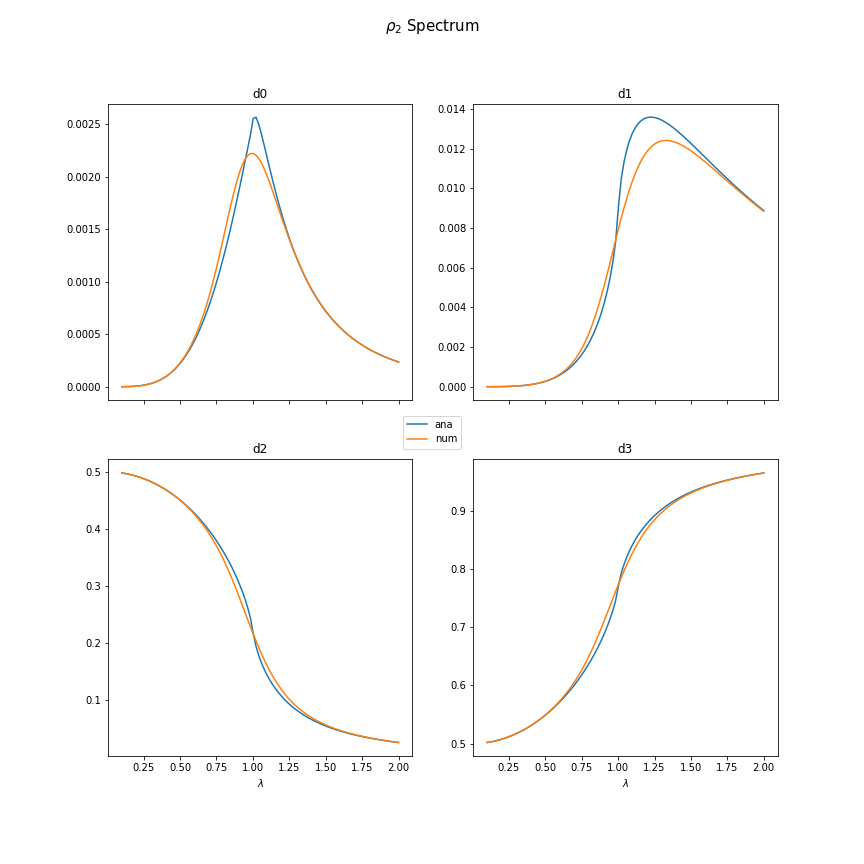
\includegraphics[width=\linewidth]{ananumwick}
		\caption{"Analitical" and "numerical" spectrum of the density matrix $\rho_2$, the eigenvalues are in ascending order. Numerical calculations on 10 sites}
		\label{fig:theoexpwick}
\end{figure}\\
Finally we can calculate the "Analitical Ergotropy": fig.\ref{fig:2siteanalerg}
\begin{figure}[h]
	\centering
	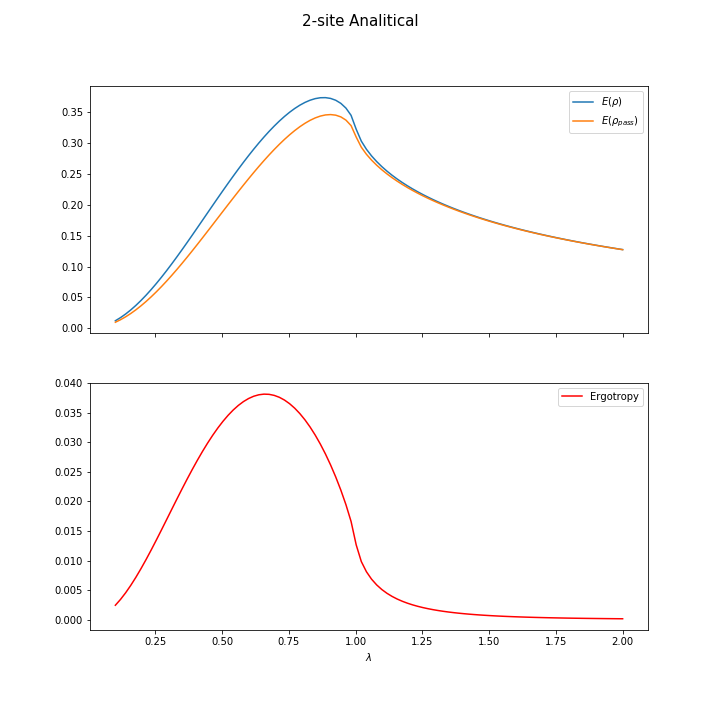
\includegraphics[width=\linewidth]{2siteanalerg}
	\caption{}
	\label{fig:2siteanalerg}
\end{figure}

	
	
	
	
	
	
	
	
	
	
	
	
	
	
	
	
	
	
	
	
	
	
	
	
	
	
	
	
	
	
	
	
	
	
	
	
	
	
	
	\subsection{Correlation Matrix derivation}\label{appendixcalculation}
	We switch to the momentum representation to exploit the translational symmetry with the help of 2N auxiliary Majorana operators:
	\begin{equation}\label{eq:ddefinition}\left[\begin{array}{c}
	\check{d}_{2 k-1} \\
	\check{d}_{2 k}
	\end{array}\right]=\sqrt{\frac{2}{N}} \sum_{l=-\frac{N-1}{2}}^{\frac{N-1}{2}} \cos \frac{2 \pi k l}{N}\left[\begin{array}{c}
	\check{a}_{2 l-1} \\
	\check{a}_{2 l}
	\end{array}\right]\end{equation}
	
	\begin{equation}\label{eq:edefinition}\left[\begin{array}{c}
	\check{e}_{2 k-1} \\
	\check{e}_{2 k}
	\end{array}\right]=\sqrt{\frac{2}{N}} \sum_{l=-\frac{N-1}{2}}^{\frac{N-1}{2}} \sin \frac{2 \pi k l}{N}\left[\begin{array}{c}
	\check{a}_{2 l-1} \\
	\check{a}_{2 l}
	\end{array}\right]\end{equation}	
	With $0\le k \le N/2$. \\
	\begin{equation}\begin{aligned}
	&\check{d}_{k}^{\dagger}=\check{d}_{k}, \quad\left\{\check{d}_{k}, \check{d}_{q}\right\}=\delta_{k q}\\
	&\check{e}_{k}^{\dagger}=\check{e}_{k}, \quad\left\{\check{e}_{k}, \check{e}_{q}\right\}=\delta_{k q}\\
	\end{aligned}	
	\end{equation} \\ 
	Using the inverse relations:
	\begin{equation}\left[\begin{array}{c}
	\check{a}_{2 l-1} \\
	\check{a}_{2 l}
	\end{array}\right]=\sqrt{\frac{2}{N}} \sum_{k=0}^{N/2} e^{-\frac{2 \pi i k l}{N}}\left[\begin{array}{c}
	\check{d}_{2 k-1}+i\check{e}_{2 k-1} \\
	\check{d}_{2 k}+i\check{e}_{2 k}
	\end{array}\right]
	\end{equation}


Substituting in \ref{eq:hamiltwitha}:
\begin{equation}\begin{aligned}
&H =\frac{i}{2} \sum_{l=-\frac{N-1}{2}}^{\frac{N-1}{2}} \check{a}_{2 l} \check{a}_{2 l+1}  
+ \lambda \check{a}_{2 l-1} \check{a}_{2 l} \\
&=\frac{i}{2}\sum_{l=-\frac{N-1}{2}}^{\frac{N-1}{2}} \frac{2}{N}\sum_{k_1=0}^{N/2} e^{\frac{2 \pi i k_1 l}{N}}   \left(\check{d}_{2 k_1}-i\check{e}_{2 k_1}\right) \sum_{k_2=0}^{N/2} e^{\frac{-2 \pi i k_2 (l+1)}{N}}  \left(\check{d}_{2 k_2-1}+i\check{e}_{2 k_2-1}  \right)  \\
&-\lambda\frac{i}{2} \frac{2}{N}\sum_{k_3=0}^{N/2} e^{\frac{2 \pi i k_3 l}{N}}   \left(\check{d}_{2 k_3}-i\check{e}_{2 k_3}\right) \sum_{k_4=0}^{N/2} e^{\frac{-2 \pi i k_4 l}{N}}  \left(\check{d}_{2 k_4-1}+i\check{e}_{2 k_4-1}  \right)\end{aligned}
\end{equation}	
Summing on $l$ first and noting that:
\begin{equation}\label{eq:delta}\begin{aligned}
&\frac{1}{N}\sum_{l=-\frac{N-1}{2}}^{\frac{N-1}{2}}e^{\frac{2 \pi i (k_1-k_2) l}{N}} = \delta_{k_1,k_2}\\
\end{aligned}
\end{equation}
we obtain:

	\begin{equation}H=\sum_{k=0}^{N / 2} H_{k} \end{equation}
		with:
		\begin{equation}
	H_k =i   \left(e^{-\frac{2\pi i k}{N}} 
	- \lambda \right)  \left(\check{d}_{2 k}-i\check{e}_{2 k}\right) \left(\check{d}_{2 k-1}+i\check{e}_{2 k-1}  \right)
	\end{equation}
			\begin{equation}
	H_k =i  \left(\cos \frac{2 \pi k }{N}-i\sin \frac{2 \pi k }{N}
	- \lambda \right)  \left(\check{d}_{2 k}\check{d}_{2 k-1}+\check{e}_{2 k}\check{e}_{2 k-1}-i\check{e}_{2k}\check{d}_{2k-1}+i\check{d}_{2k}\check{e}_{2k-1}\right) 
	\end{equation}

	\begin{equation}H_{k}=\frac{i\Lambda_k}{2}\left[\begin{array}{c}
	\check{d}_{2 k-1} \\
	\check{e}_{2 k-1} \\
	\check{d}_{2 k} \\
	\check{e}_{2 k}
	\end{array}\right]^{T}\left[\begin{array}{cccc}
	0 & 0 & c_{k} & -s_{k} \\
	0 & 0 & s_{k} & c_{k} \\
	-c_{k} &-s_{k} & 0 & 0 \\
	s_{k} &- c_{k} & 0 & 0
	\end{array}\right]\left[\begin{array}{c}
	\check{d}_{2 k-1} \\
	\check{e}_{2 k-1} \\
	\check{d}_{2 k} \\
	\check{e}_{2 k}
	\end{array}\right]\end{equation}
	\newline
	\begin{equation}
	\begin{aligned}
&\Lambda_k \equiv\sqrt{\left(\cos \frac{2 \pi k }{N}-\lambda\right)^2+\sin^2 \frac{2 \pi k }{N}}
\\
&c_{k}\equiv\left(\lambda-\cos \frac{2 \pi k }{N}\right)/\Lambda_k
\\
&s_{k}\equiv\left(-\sin \frac{2 \pi k }{N}\right)/\Lambda_k
	\end{aligned}
	\end{equation}\\
Since by construction $c_k^2+s_k^2=1$,
 $\left[\begin{array}{cccc}
0 & 0 & c_{k} & -s_{k} \\
0 & 0 & s_{k} & c_{k} \\
-c_{k} &-s_{k} & 0 & 0 \\
s_{k} &- c_{k} & 0 & 0\end{array}\right]^2 =-I$ \\
So it exist an orthogonal transformation that defines new operators $\check{b}_{p},  -N\le p \le N-1$ :

\begin{equation}\label{eq:orthogonal}\left[\begin{array}{c}
\check{b}_{-2 k-1} \\
\check{b}_{-2 k} \\
\check{b}_{2 k-1} \\
\check{b}_{2 k}
\end{array}\right]=\frac{1}{\sqrt{2}}\left[\begin{array}{cccc}
u_{k} & v_{k} & u_{k} & -v_{k} \\
u_{k} & v_{k} & -u_{k} & v_{k} \\
v_{k} & -u_{k} & v_{k} & u_{k} \\
-v_{k} & u_{k} & v_{k} & u_{k}
\end{array}\right]\left[\begin{array}{c}
\check{d}_{2 k-1} \\
\check{e}_{2 k-1} \\
\check{d}_{2 k} \\
\check{e}_{2 k}
\end{array}\right]\end{equation}	
and puts the Hamiltonian in the block diagonal form (canonical form for a skew-symmetric matrix):
\begin{equation}H=\frac{i}{2} \sum_{k=-\frac{N-1}{2}}^{\frac{N-1}{2}} \Lambda_k\left(\tilde{b}_{2 k-1} \tilde{b}_{2 k}-\tilde{b}_{2 k} \tilde{b}_{2 k-1}\right)=
\frac{i}{2}\bigoplus_{k=-\frac{N-1}{2}}^{\frac{N-1}{2}} \Lambda_k\left[\begin{array}{cc}
0 & 1 \\
-1 & 0
\end{array}\right]\end{equation}	
For one moment we switch to non-Hermitian fermionic operators:
\begin{equation}\hat{b}_{k} \equiv \frac{\check{b}_{2 k-1}+i \check{b}_{2 k}}{2}\end{equation}
\begin{equation}
H= \sum_{k=-\frac{N-1}{2}}^{\frac{N-1}{2}} \Lambda_k\hat{b}_k^\dagger\hat{b}_k-\Lambda_k/2
\end{equation}
The second term is a constant and can be ignored.\\
Now since all $\Lambda_k>0$ we can finally find the ground state imposing
$b_k\ket{ \psi_g}=0$ \\ From which also: $\hat{b}_k^\dagger \hat{b}_k\ket{ \psi_g}=\hat{b}_k \hat{b}_k\ket{ \psi_g}=0$ and  $b_k \hat{b}_k^\dagger\ket{\psi_g}=\ket{\psi_g}$ \\
Using as always the inverse transformations we can calculate the correlation matrix on the ground state for the Majorana operators:
\begin{equation}\begin{split}
&<\check{b}_{2k-1}\check{b}_{2k}>=i<\hat{b}_k\hat{b}_k^\dagger>=i\\ &<\check{b}_{2k}\check{b}_{2k-1}>=-i<\hat{b}_k\hat{b}_k^\dagger>=-i \\&<\check{b}_{2k}\check{b}_{2k}>=<\check{b}_{2k-1}\check{b}_{2k-1}>=<\hat{b}_k\hat{b}_k^\dagger>=1\\
\end{split}
\end{equation}\\
In compact notation:
\begin{equation}
\left\langle\check{b}_{p} \check{b}_{q}\right\rangle=\delta_{p q}+i \Gamma_{p q}^{B}
\end{equation}

\begin{equation}\label{eq:corrmatrb}\Gamma^{B}=\bigoplus_{k=-\frac{N-1}{2}}^{\frac{N-1}{2}}\left[\begin{array}{rr}
0 & 1 \\
-1 & 0
\end{array}\right]\end{equation}
Now that we have the correlation matrix for the $\check{b}$ operators we have to go back to the $\check{a}$, that means we have to find the matrix $W$:
\begin{equation}\label{eq:wmatrix}\check{b}_{p}=\sum_{m=-N}^{N-1} W_{p m} \check{a}_{m}, \quad-N+1 \leq p \leq N\end{equation}
The orthogonal transformation that defines the $\check{b}$ operators:
\begin{equation}\label{eq:orthogonal2}\left[\begin{array}{c}
\check{b}_{-2 k-1} \\
\check{b}_{-2 k} \\
\check{b}_{2 k-1} \\
\check{b}_{2 k}
\end{array}\right]=\frac{1}{\sqrt{2}}\left[\begin{array}{cccc}
u_{k} & v_{k} & u_{k} & -v_{k} \\
u_{k} & v_{k} & -u_{k} & v_{k} \\
v_{k} & -u_{k} & v_{k} & u_{k} \\
-v_{k} & u_{k} & v_{k} & u_{k}
\end{array}\right]\left[\begin{array}{c}
\check{d}_{2 k-1} \\
\check{e}_{2 k-1} \\
\check{d}_{2 k} \\
\check{e}_{2 k}
\end{array}\right]\end{equation}
has coefficients $u_k=\cos(\theta_k/2)$, $v_k=\sin(\theta_k/2)$ such that:
\begin{equation}\begin{aligned}
&u_k^2-v_k^2=\cos(\theta_k)=\left(\lambda-\cos \frac{2 \pi k }{N}\right)/\Lambda_k\\
&2u_kv_k=\sin(\theta_k)=\left(-\sin \frac{2 \pi k }{N}\right)/\Lambda_k\\
\end{aligned}
\end{equation} 
For the sake of clarity we split the transformation \ref{eq:orthogonal2} in two even and odd parts:
\begin{equation}\label{eq:orthogonaevenodd}\left[\begin{array}{c}
\check{b}_{-2 k-1} \\
\check{b}_{-2 k} \\
\check{b}_{2 k-1} \\
\check{b}_{2 k}
\end{array}\right]=\frac{1}{\sqrt{2}}\left[\begin{array}{cc}
u_{k} & v_{k}  \\
u_{k} & v_{k}  \\
v_{k} & -u_{k} \\
-v_{k} & u_{k} 
\end{array}\right]\left[\begin{array}{c}
\check{d}_{2 k-1} \\
\check{e}_{2 k-1} 
\end{array}\right]+\frac{1}{\sqrt{2}}\left[\begin{array}{cc}
u_{k} & -v_{k}  \\
-u_{k} & v_{k}  \\
v_{k} & u_{k} \\
v_{k} & u_{k} 
\end{array}\right]\left[\begin{array}{c}
\check{d}_{2 k} \\
\check{e}_{2 k} 
\end{array}\right]\end{equation}\\
and now using the definitions of $\check{d}$ and $\check{e}$ ( \ref{eq:ddefinition} , \ref{eq:edefinition} ):
\begin{equation}\label{eq:orthogonalba}\left[\begin{array}{c}
\check{b}_{-2 k-1} \\
\check{b}_{-2 k} \\
\check{b}_{2 k-1} \\
\check{b}_{2 k}
\end{array}\right]=\frac{1}{\sqrt{N}}\sum_{l=-\frac{N-1}{2}}^{\frac{N-1}{2}}\left(\left[\begin{array}{cc}
u_{k} & v_{k}  \\
u_{k} & v_{k}  \\
v_{k} & -u_{k} \\
-v_{k} & u_{k} 
\end{array}\right]\left[\begin{array}{c}
 \cos \frac{2 \pi k l}{N}  \\
 \sin \frac{2 \pi k l}{N}  
\end{array}\right]\check{a}_{2l-1}+
\left[\begin{array}{cc}
u_{k} & -v_{k}  \\
-u_{k} & v_{k}  \\
v_{k} & u_{k} \\
v_{k} & u_{k} 
\end{array}\right]\left[\begin{array}{c}
\cos \frac{2 \pi k l}{N}  \\
\sin \frac{2 \pi k l}{N}  
\end{array}\right]\check{a}_{2l}\right) \end{equation}
With this equation \ref{eq:orthogonalba} we can read the coefficients of $W$ as defined in \ref{eq:wmatrix}.
\newline
The correlation matrix $\Gamma^A$ for the operators $\check{a}$ is given by:
\begin{equation}
\Gamma^A=W^T\Gamma^BW
\end{equation}
Using the definition of $\Gamma^B$ \ref{eq:corrmatrb}:
\begin{equation}\label{eq:corrmatra}
\Gamma^A_{mn}= \sum_{i,j}  W^T_{mi} \Gamma^B_{ij} W_{jn}=\sum_{k=-\frac{N-1}{2}}^{\frac{N-1}{2}} W^T_{m , 2k-1}W_{2k,n}-W^T_{m , 2k}W_{2k-1,n}=\sum_{k=-\frac{N-1}{2}}^{\frac{N-1}{2}}  W_{2k-1,m}W_{2k,n}-W_{2k , m}W_{2k-1,n}
\end{equation}\\
Now using \ref{eq:orthogonalba} and \ref{eq:corrmatra} we explicitly calculate an element of the correlation $\Gamma^A$ :
\begin{equation}\begin{aligned}\label{eq:finiten}
&<\check{a}_{2m-1}\check{a}_{2n}>=\Gamma^A_{2m-1,2n}=\sum_{k=-\frac{N-1}{2}}^{\frac{N-1}{2}}  W_{2k-1,2m-1}W_{2k,2n}-W_{2k , 2m-1}W_{2k-1,2n}=\\
&\sum_{k=1}^{\frac{N-1}{2}}\left(  W_{2k-1,2m-1}W_{2k,2n}-W_{2k , 2m-1}W_{2k-1,2n}+W_{-2k-1,2m-1}W_{-2k,2n}-W_{-2k , 2m-1}W_{-2k-1,2n}\right)+ \\&W_{-1,2m-1}W_{0,2n}-W_{-1 , 2m-1}W_{0,2n}=\\
&=\frac{2}{N}\sum_{k=1}^{\frac{N-1}{2}}\left(v_k \cos \frac{2 \pi k m}{N}-u_k\sin \frac{2 \pi k m}{N}\right)\left(v_k\cos \frac{2 \pi k n}{N}+u_k\sin \frac{2 \pi k n}{N}\right)+\\& \left(u_k \cos \frac{2 \pi k m}{N}+v_k\sin \frac{2 \pi k m}{N}\right)\left(v_k\sin \frac{2 \pi k n}{N}-u_k\cos \frac{2 \pi k n}{N}\right)-u_0^2= \\
&\frac{2}{N}\sum_{k=0}^{\frac{N}{2}}\cos(\theta_k)\cos{\frac{2\pi k (m-n)}{N}}-\sin(\theta_k)\sin{\frac{2\pi k (m-n)}{N}}\\\\
\end{aligned}	
\end{equation}
Now calling $\phi \equiv \frac{2\pi k}{N}$ and sending $N\rightarrow\infty$:
\begin{equation}
<\check{a}_{2m-1}\check{a}_{2n}>=\frac{1}{\pi}\int_{0}^{\pi}d\phi    \frac{\lambda-\cos\phi}{|\lambda-\cos\phi+i\sin\phi|}\cos{\phi(m-n)}-\frac{1}{\pi}\int_{0}^{\pi}d\phi \frac{\sin\phi}{|\lambda-\cos\phi+i\sin\phi|}\sin{\phi(m-n)}
\end{equation}
Wich can be written in the more compact form:
\begin{equation}
<\check{a}_{2m-1}\check{a}_{2n}>=\frac{1}{2\pi}\int_{0}^{2\pi}d\phi \  e^{-i \phi  (n-m)} \frac{\lambda-\cos\phi+i\sin\phi}{|\lambda-\cos\phi+i\sin\phi|}
\end{equation}
\newpage
\subsection{DMRG calculations}
In fig. \ref{fig:theoexpwick} we noticed a difference between the "analytical" and the "numerical" spectrum of $\rho_2$. This difference is due to two factors:
\begin{enumerate}
	\item Finite Size: the analytical calculations are carried on for $N\rightarrow\infty$, the numerical simulations on a finite chain ($N=10$)
	\item Boundary conditions: For the calculations we applied Open Boundary Conditions, the simulation uses Periodic Boundary Conditions
\end{enumerate} 
The second factor becomes important at small sizes.\\
Now we have two ways to go:
\begin{enumerate}
\item adapt the analytical calculation to our limited size and different boundary condition 
\item increase the size and change the boundary conditions of the simulations
\end{enumerate}
For now we will go down the second path and use the Density Matrix Renormalization Group \cite{PhysRevLett.69.2863}.\\
DMRG is a numerical algorithm that it's able to obtain with high precision the ground state of 1D lattices, for Ising chains \ref{eq:hamilt} we can go up to hundreds of sites,
DMRG  works better for systems with Open Boundary Conditions.\\
The key part of the DMRG is the "decimation procedure" that selects the "most probable" states of the system. The success of the algorithm depends on the amount of entanglement between a subsystem and the rest of the lattice in the ground state. \cite{De_Chiara_2008}.\\
Some results are in fig. \ref{fig:dmrg3020} and \ref{fig:dmrg6020} , there are almost no differences between the predicted and simulated eigenvalues of $\rho_2$, that means that the calculations in sec. \ref{sec:analerg} are correct. \\

\subsubsection{Technical note}\label{sec:technicdmrg}
I used the Infinite-system DMRG for the simulation. The algorithm failed to capture the symmetry in $\lambda=0$ and returned ($\ket{\rightarrow\rightarrow\rightarrow}$ and $\ket{\leftarrow\leftarrow\leftarrow}$) as two states with different energy so i decided to compute the first two energy levels (let's call them $\psi_g$ and $\psi_e$ ) and use $\rho_{eff}=\frac{1}{2}\rho_g+\frac{1}{2}\rho_e$ as $\rho_2$ when $\lambda<1$. This way i'm forcing the algorithm to consider as equally likely the first two states. Maybe using the finite-system DMRG could have solved the problem in "cleaner" way.

\begin{figure}[b]
	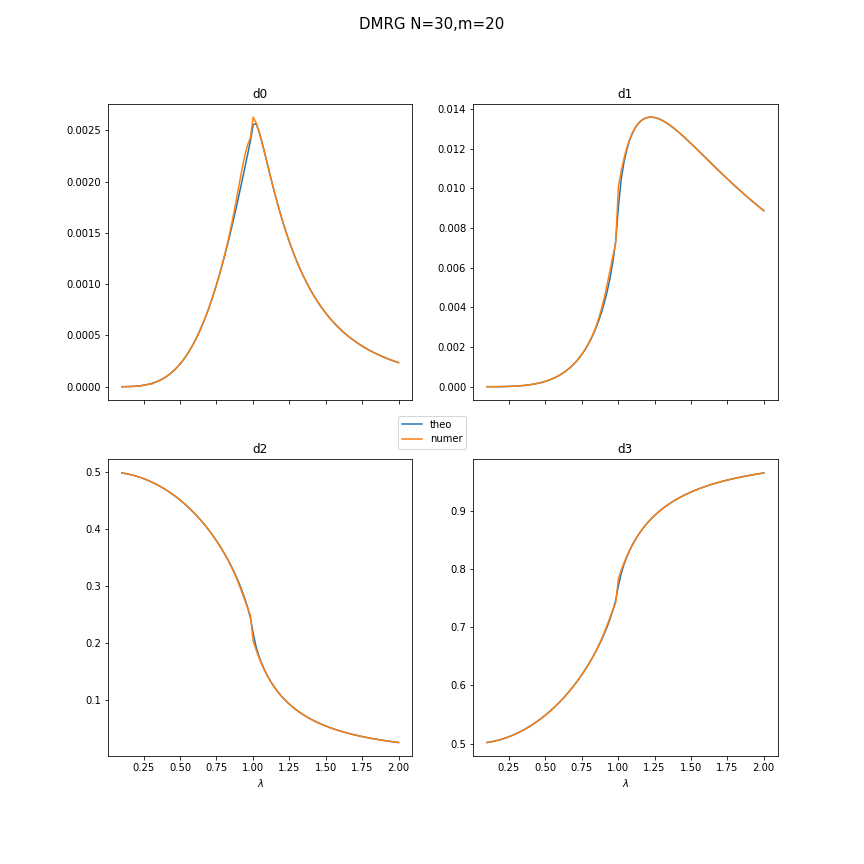
\includegraphics[width=\linewidth]{dmrg3020}
	\caption{Predicted and simulated eigenvalues of $\rho_2$, simulations done with i-DMRG on a lattice with 30 sites and keeping the first m=20 eigenstates.}
	\label{fig:dmrg3020}
\end{figure}
\begin{figure}[b]
	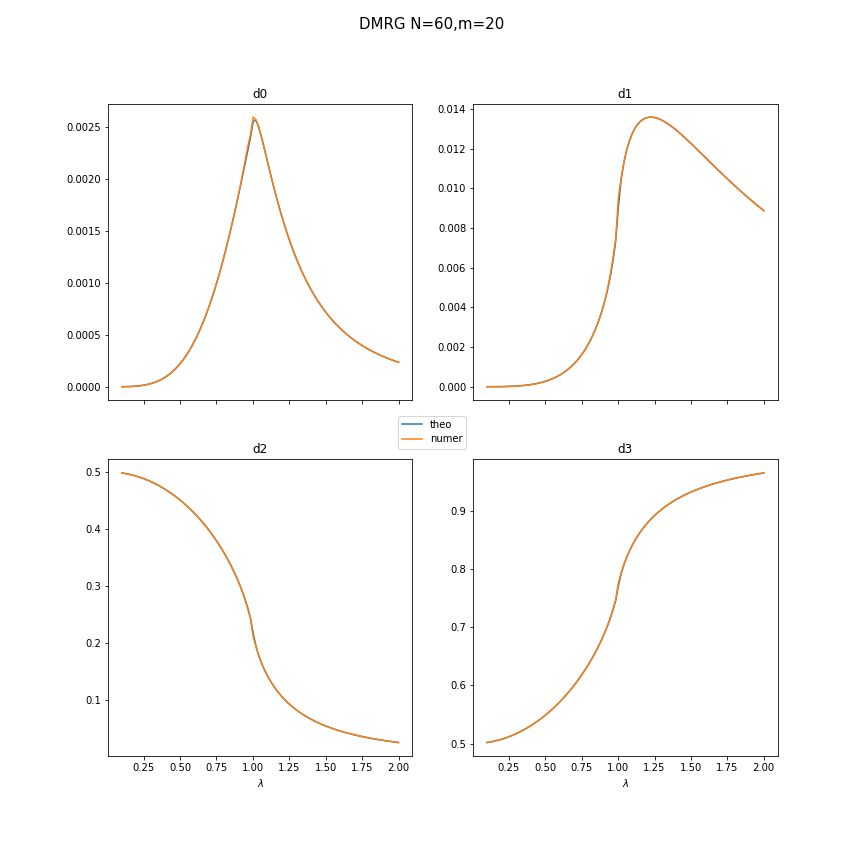
\includegraphics[width=\linewidth]{dmrg6020}
	\caption{Predicted and simulated eigenvalues of $\rho_2$, simulations done with i-DMRG on a lattice with 60 sites and keeping the first m=20 eigenstates.}
	\label{fig:dmrg6020}
\end{figure}

\subsection{L-site density matrix}\label{sec:L-site}
In sec. \ref{sec:2sitecoff}, we obtained the 2-site density matrix of the ground state \ref{eq:rho2}. The most time-consuming part of the calculation was the derivation of the coefficients 	$\rho_{\mu_{1}  \mu_{2}}=\left\langle\sigma_{1}^{\mu_{1}}  \sigma_{2}^{\mu_{2}}\right\rangle$ defined in \ref{2sitepauli} 
and obtained in \ref{eq:coeff2sites} via Wick expansion.\\
To repeat the same derivation for a L-site matrix we have to calculate in the same way the coefficients \ref{eq:rhoexpansion} :
\begin{equation}\rho_{\mu_{1}\cdots  \mu_{L}}=\left\langle\sigma_{1}^{\mu_{1}}\cdots  \sigma_{L}^{\mu_{L}}\right\rangle  \qquad \mu_{L}=0, x, y, z\end{equation}
so $2^{2L}$ Wick expansions as in \ref{eq:wickcalc} .\\
It can be shown that the symmetry \ref{eq:symm} halves the number of non-zero coefficients to $2^{2L-1}$.
Nevertheless, the scaling is exponential so we will calculate the coefficients for the 3-site density matrix with the help of a computer.
\subsubsection{3-site density matrix}
We want  to calculates the expectations values on the ground state:
\begin{equation}\rho_{\mu_{1}\mu_2  \mu_{3}}=\left\langle\sigma_{1}^{\mu_{1}}\sigma_{2}^{\mu_{2}} \sigma_{3}^{\mu_{3}}\right\rangle  \qquad \mu_{L}=0, x, y, z\end{equation}
(subscripts label the site) \ref{eq:rhoexpansion} \\
As noted in sec \ref{sec:L-site} the simmetry \ref{eq:symm} brings down the number of coefficient to $2^{5}=32$.

We will exclude the ones with $\mu_{3}=0$ , since they reduce to the 2-site ones  we already calculated in sec. \ref{sec:2sitecoff} . 
Using the computer we find that there are 24 amplitudes to be contracted:\\
\begin{equation}\label{eq:3-sitecoeff}
\begin{aligned}
&IIZ, IXX, IXY, IYX, IYY, IZZ, XIX, XIY, XXZ, XYZ, XZX, XZY, \\&  YIX, YIY, YXZ, YYZ, YZX, YZY, ZIZ, ZXX, ZXY, ZYX, ZYY, ZZZ
\end{aligned}
\end{equation}

As for the 2-site derivation (\ref{eq:corrmatr2sites1}, \ref{eq:corrmatrrestrict} \ref{eq:corrmatr3}) we write
the correlation matrix for the majorana operators on three sites:
\begin{equation}\label{eq:corrmatr3sites1}
\left\langle\check{a}_{m} \check{a}_{n}\right\rangle=\delta_{m n}+i\left(\Gamma_{3}^{A}\right)_{m n}, \quad m, n=1,2,3,4,5,6
\end{equation}
\begin{equation}\label{eq:corrmatr3sites2}
\Gamma_{3}^{A}=\left[\begin{array}{ccc}
\Pi_0 & \Pi_1 &\Pi_2\\
-\Pi_1^T & \Pi_0& \Pi_1\\
-\Pi_2^T & -\Pi_1^T& \Pi_0\\
\end{array}\right] 
\end{equation}

\begin{equation}
\Pi_{l}=\left[\begin{array}{cc}
0 & g_{l} \\
-g_{-l} & 0
\end{array}\right] 
\quad g_{l}=\frac{1}{2 \pi} \int_{0}^{2 \pi} d \phi e^{-i l \phi} \frac{\lambda-\cos \phi+i \sin \phi}{|\lambda-\cos\phi +i  \sin \phi|}\end{equation}

And we will need again the transformations: \ref{eq:inversez}-\ref{eq:inversey}

\begin{equation}
\sigma_{l}^{z} = -i\check{a}_{2l-1} \check{a}_{2 l} 
\end{equation}
\begin{equation}
\sigma_{l}^{x}= \left(\prod_{m<l} \sigma_{m}^{z}\right)\check{a}_{2l-1}=
\left(\prod_{m<l} -i\check{a}_{2l-1} \check{a}_{2 l}\right)\check{a}_{2l-1}
\end{equation}
\begin{equation}
\sigma_{l}^{y}=
\left(\prod_{m<l} -i\check{a}_{2l-1} \check{a}_{2 l}\right)\check{a}_{2l}
\end{equation}
Now (with the computer) we have to express the coefficients \ref{eq:3-sitecoeff} in the Majorana basis, perform the wick contractions and read the expectaction values from the correlation matrix \ref{eq:corrmatr3sites1}.\\
For example the first two:\\
\begin{equation}
\rho_{00z}=\left\langle\sigma_{1}^{0}\sigma_{2}^{0} \sigma_{3}^{z}\right\rangle=-i\left\langle\check{a}_{5} \check{a}_{6}\right\rangle=g_{-2}
\end{equation} 
\begin{equation}\begin{aligned}\label{eq:esempiol3}
&\rho_{0xx}=\left\langle\sigma_{1}^{0}\sigma_{2}^{x} \sigma_{3}^{x}\right\rangle=-i\left\langle\check{a}_1
\check{a}_2
\check{a}_3
\check{a}_1
\check{a}_2
\check{a}_3
\check{a}_4
\check{a}_5\right\rangle=-i\left\langle\check{a}_1
\check{a}_4\right\rangle\left\langle
\check{a}_2
\check{a}_1\right\rangle\left\langle
\check{a}_2
\check{a}_5\right\rangle\left\langle
\check{a}_3
\check{a}_3 \right\rangle \\ &\text{ and other 27 non-zero contraction terms}
\end{aligned}
\end{equation}
%
%\begin{equation}
%\begin{aligned}
%& \rho_3=\frac{1}{8} \left( \rho_{ iiz } \left( \sigma_1^i \otimes \sigma_2^i \otimes \sigma_3^z \right) +
%\rho_{ ixx } \left( \sigma_1^i \otimes \sigma_2^x \otimes \sigma_3^x \right) +
%\rho_{ ixy } \left( \sigma_1^i \otimes \sigma_2^x \otimes \sigma_3^y \right) +
%\rho_{ iyx } \left( \sigma_1^i \otimes \sigma_2^y \otimes \sigma_3^x \right) + \\
%& \rho_{ iyy } \left( \sigma_1^i \otimes \sigma_2^y \otimes \sigma_3^y \right) +
%\rho_{ izz } \left( \sigma_1^i \otimes \sigma_2^z \otimes \sigma_3^z \right) +
%\rho_{ xix } \left( \sigma_1^x \otimes \sigma_2^i \otimes \sigma_3^x \right) + 
%\rho_{ xiy } \left( \sigma_1^x \otimes \sigma_2^i \otimes \sigma_3^y \right) + \\
%&
%\rho_{ xxz } \left( \sigma_1^x \otimes \sigma_2^x \otimes \sigma_3^z \right) +
%\rho_{ xyz } \left( \sigma_1^x \otimes \sigma_2^y \otimes \sigma_3^z \right) + \rho_{ xzx } \left( \sigma_1^x \otimes \sigma_2^z \otimes \sigma_3^x \right) +  
%\rho_{ xzy } \left( \sigma_1^x \otimes \sigma_2^z \otimes \sigma_3^y \right) +\\
%&
%\rho_{ yix } \left( \sigma_1^y \otimes \sigma_2^i \otimes \sigma_3^x \right) +
%\rho_{ yiy } \left( \sigma_1^y \otimes \sigma_2^i \otimes \sigma_3^y \right) +
%\rho_{ yxz } \left( \sigma_1^y \otimes \sigma_2^x \otimes \sigma_3^z \right) +
%\rho_{ yyz } \left( \sigma_1^y \otimes \sigma_2^y \otimes \sigma_3^z \right) +\\
%&
%\rho_{ yzx } \left( \sigma_1^y \otimes \sigma_2^z \otimes \sigma_3^x \right) +
%\rho_{ yzy } \left( \sigma_1^y \otimes \sigma_2^z \otimes \sigma_3^y \right) +
%\rho_{ ziz } \left( \sigma_1^z \otimes \sigma_2^i \otimes \sigma_3^z \right) +
%\rho_{ zxx } \left( \sigma_1^z \otimes \sigma_2^x \otimes \sigma_3^x \right) +\\
%&
%\rho_{ zxy } \left( \sigma_1^z \otimes \sigma_2^x \otimes \sigma_3^y \right) +
%\rho_{ zyx } \left( \sigma_1^z \otimes \sigma_2^y \otimes \sigma_3^x \right) +
%\rho_{ zyy } \left( \sigma_1^z \otimes \sigma_2^y \otimes \sigma_3^y \right) +
%\rho_{ zzz } \left( \sigma_1^z \otimes \sigma_2^z \otimes \sigma_3^z \right) \right) \\
%\end{aligned}
%\end{equation}
\section{Commenti}
Ho reso più esplicita la derivazione della matrice di correlazione in \ref{appendixcalculation} per cercare di studiare analiticamente il caso N finito, ho cominciato le simulazioni con il DMRG e sto calcolando i coefficienti per L=3. Potrebbe essere utile provare ad utilizzare un algoritmo finite-DMRG invece che Infinite-DMRG come accennato in \ref{sec:technicdmrg} ?\\
Provo a rispondere ad alcune domande:
\begin{itemize}
\item  Per una catena di lunghezza finita, siamo in grado di calcolare analiticamente la matrice densita? \\
Se lascio il numero di siti N finito in \ref{eq:finiten} ( in pratica basta sostituire $\phi=\frac{2\pi k}{N}$ in tutte le formule), gli autovalori di $\rho_2$ non corrispondono a quelli delle simulazioni. Non so bene perché ma credo sia dovuto al fatto che a taglia finita il sistema non è invariante per traslazione e ad esempio forse non potremmo effettuare la trasformata di fourier in \ref{eq:ddefinition}
\item  Possiamo utilizzare solo lo spettro di $\rho_2$ (quindi evitare di calcolare tutta la matrice come in \ref{eq:rho2} ) per calcolare l'ergotropia?\\
 Se ci fosse un metodo per farlo il conto sarebbe sicuramente più facile in quanto come mostrato in \cite{latorre2003ground} si fa molto prima ad ottenere solo gli autovalori di $\rho_L$ senza gli autovettori. Per calcolare l'ergotropia ho utilizzato la formula \ref{eq:ergotropy2} : se per calcolare $E(\rho_{pass})$ bastano gli autovalori di $\rho$, non credo si possa calcolare $E(\rho)$ senza conoscere gli autovettori di $\rho$. L'ergotropia in \cite{allahverdyan2004maximal} è definita proprio come: \begin{equation}\mathcal{W}=\sum_{j, k} r_{j} \varepsilon_{k}\left(\left|\left\langle r_{j} \mid \varepsilon_{k}\right\rangle\right|^{2}-\delta_{j k}\right)\end{equation} 
dove $\ket{r_j}$ sono gli autovettori di $\rho$.\\
In effetti finora ho controllato solo la corrispondenza degli autovalori tra calcolo analitico e numerico, credo sarebbe utile verificare anche l'uguaglianza degli autovettori.

\item Come scala con la taglia della matrice densita il costo computazionale?\\
Come ho accennato in \ref{sec:L-site} purtroppo scala in maniera esponenziale. Il programmino che ho scritto ( sicuramente non ottimizzato perfettamente) mi permette di calcolare in circa 2 secondi tutte le contrazioni per L=3 (come quelle in  \ref{eq:esempiol3} ) ma per L=4 mi sembra difficile riuscire a calcolare qualcosa.
Ad esempio già per L=3 il termine (le lettere indicano le matrici sigma e i numeri la loro espressione in operatori di majorana): $\left\langle zyx\right\rangle=\left\langle1212412345\right\rangle$ 
ha 703 contrazioni non banalmente nulle. (una contrazione banalmente nulla è una che contiene un elemento di matrice nullo).\\
Risulta evidente che il  problema non è solo la crescita del numero di correlatori ma anche (e sopratutto) che a lunghezza crescente bisogna effettuare più contrazioni.\\
Forse c'è un metodo di procedere più efficiente, intanto la settimana prossima (fino a lunedì 21/09 non avrò accesso al computer) proverò a calcolare la matrice densità per L=3 .

\item Come si può generalizzare il conto al modello XY?\\
Non credo sia particolarmente difficile, seguendo \cite{latorre2003ground} se 

\begin{equation}
		H_{X Y} =-\frac{1}{2} \sum_{l=-\frac{N-1}{2}}^{\frac{N-1}{2}}\left(\frac{1+\gamma}{2} \sigma_{l}^{x} \sigma_{l+1}^{x}+\frac{1-\gamma}{2} \sigma_{l}^{y} \sigma_{l+1}^{y}\right)
		-\frac{1}{2} \sum_{l=-\frac{N-1}{2}}^{\frac{N-1}{2}} \lambda \sigma_{l}^{z}
\end{equation}
(Il modello di Ising \ref{eq:hamilt} è l'XY a $\gamma=1$)\\
Basta trasformare i $g_l$:
\begin{equation}
g_{l}=\frac{1}{2 \pi} \int_{0}^{2 \pi} d \phi e^{-i l \phi} \frac{\lambda-\cos \phi+i \sin \phi}{|\lambda-\cos\phi +i  \sin \phi|} \rightarrow \frac{1}{2 \pi} \int_{0}^{2 \pi} d \phi e^{-i l \phi} \frac{\lambda-\cos \phi+i \gamma \sin \phi}{|\lambda-\cos\phi +i  \sin \phi|}
\end{equation}
e poi il resto del conto è uguale.

\end{itemize}
\clearpage
\section{L=1 Calculations}
There are only two Majorana fermions: $\check{a}_1$ and $\check{a}_2$.\\
The one-site Hamiltonian is $-\frac{\lambda}{2}\sigma^z$\\
We write all the correlators in the form $\delta_{m n}+i\Gamma_{m n}$:
\begin{equation}
	\langle\check{a}_{m} \check{a}_{n}\rangle= \left[\begin{array}{cc}
		1 & 0 \\
		0 & 1
	\end{array}\right]+i\left[\begin{array}{cc}
	0 & g_0 \\
	-g_0 & 0
\end{array}\right]
\end{equation}
$\Gamma$ is already in the block diagonal form.\\
The density matrix $\rho_1$ has eigenvalues:
\begin{equation}
	p_1=(1+g_0)/2 \quad p_2=(1-g_0)/2
\end{equation}\\
With $g_0$:
\begin{equation}
	g_0=\frac{1}{2 \pi} \int_{0}^{2 \pi} d \phi \frac{\lambda-\cos \phi+i \sin \phi}{|\lambda-\cos\phi +i  \sin \phi|}=\frac{1}{2 \pi} \int_{0}^{2 \pi} d \phi \frac{\lambda-\cos \phi}{\sqrt{(\lambda-\cos\phi)^2 +  \sin^2 \phi}}
\end{equation}
\begin{figure}[h!]
	\centering
	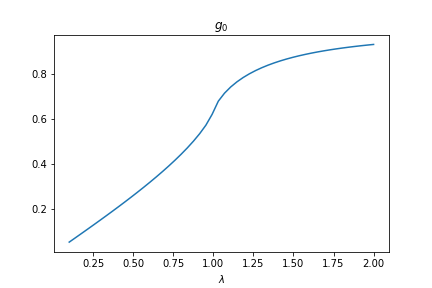
\includegraphics[width=0.7\linewidth]{g0}
	\caption{}
	\label{fig:g0}
\end{figure}\\
\begin{figure}[h!]
	\centering
	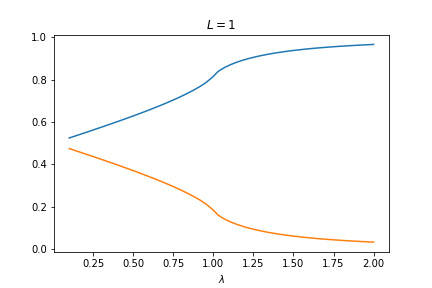
\includegraphics[width=0.7\linewidth]{L1_lambda}
	\caption{Eigenvalues of one-site density matrix}
	\label{fig:l1lambda}
\end{figure}\\
From the eigenvalues we can already calculate something:
\begin{itemize}
	\item Purity: 

	\begin{equation}
		\mathfrak{P}(1)=\sum_{i}\left(p_{i}\right)^{2}=\frac{1+g_0^2}{2}
	\end{equation}
	\item Max-Ergo:
	
	\begin{equation}
			\mathcal{M}(1)=2 \sum_{i=1}^{D / 2}\left(p_{i}^{(\downarrow)}-p_{D-i+1}^{(\downarrow)}\right)\left|\epsilon_{i}^{(\uparrow)}\right|=2(p_1-p_2)\abs{e_1}=2g_0\abs{\frac{\lambda}{2}}
	\end{equation}
	\item Rescaled-Max-Ergo
	\begin{equation}
	\mathfrak{M}(\mathcal{I})=g_0
	\end{equation}	
	
\end{itemize}
\begin{figure}[h]
	\centering
	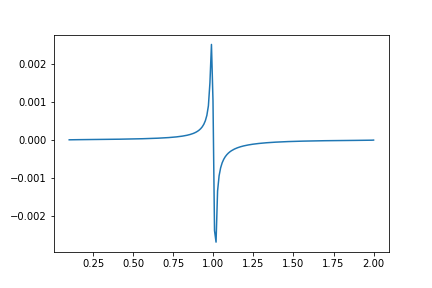
\includegraphics[width=0.7\linewidth]{one_site_secdev}
	\caption{Second Derivative Ergotropy ($g_0$)}
	\label{fig:onesitesecdev}
\end{figure}

\section{Two sites}

Eigenvalues of the correlation matrix
\begin{equation}
	\nu_{\pm}=\sqrt{\left(\frac{g_{1}-g_{-1}}{2}\right)^{2}+g_{0}^{2}} \pm \left| \frac{g_{1}+g_{-1}}{2} \right|
\end{equation}
$\nu_-<\nu_+$\\
\begin{figure}[h]
	\centering
	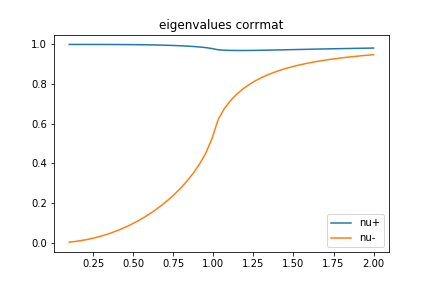
\includegraphics[width=0.7\linewidth]{nuplot}
	\caption{}
	\label{fig:nuplot}
\end{figure}
\begin{equation}
	\left\langle\hat{c}_{m} \hat{c}_{n}\right\rangle=0, \quad\left\langle\hat{c}_{m}^{\dagger} \hat{c}_{n}\right\rangle=\delta_{m n} \frac{1+\nu_{m}}{2}
\end{equation}
\begin{equation}
	\left\langle g\left|c_{j}^{\dagger} c_{j}\right| g\right\rangle=\frac{1+\nu_{j}}{2}
\end{equation}
Eigenvalues of the density matrix:
\begin{equation}
	p_{\pm \pm } =(1 \pm \nu_-)(1 \pm \nu_+)/4
\end{equation}
\begin{figure}[h]
	\centering
	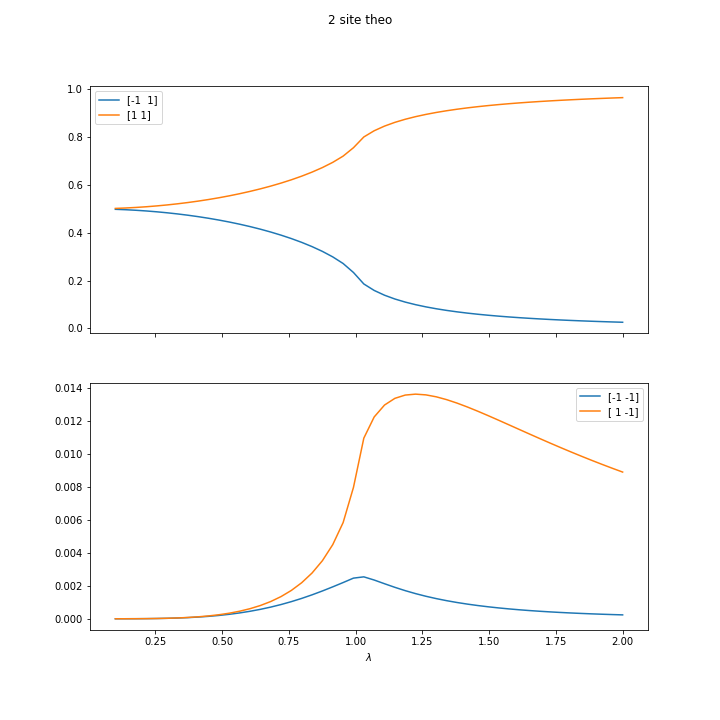
\includegraphics[width=0.7\linewidth]{two_site_theo}
	\caption{Eigenvalues of the 2-site density matrix}
	\label{fig:twositetheo}
\end{figure}

Eigenvalues of 2 site Hamiltonian:
\begin{equation}
	H=-\frac{1}{2} \left(\sigma^{x} \sigma^{x}+\lambda\sigma^{z} \sigma^0+\lambda\sigma^0\sigma^{z}\right) =
	\left(
	\begin{array}{cccc}
		-\lambda  & 0 & 0 & -\frac{1}{2} \\
		0 & 0 & -\frac{1}{2} & 0 \\
		0 & -\frac{1}{2} & 0 & 0 \\
		-\frac{1}{2} & 0 & 0 & \lambda  \\
	\end{array}
	\right)
\end{equation}
\begin{equation}
	\left\{-\frac{1}{2} \sqrt{1+4 \lambda ^2},-\frac{1}{2},\frac{1}{2},,\frac{1}{2} \sqrt{1+4 \lambda ^2}\right\}
\end{equation}

\begin{equation}
	\begin{aligned}
		&
		\mathcal{M}(\mathcal{I})=2 \sum_{i=1}^ {2}\left(p_{i}^{(\downarrow)}-p_{D-i+1}^{(\downarrow)}\right)\left|\epsilon_{i}^{(\uparrow)}\right|	\\
		& \left(p_{1}^{(\downarrow)}-p_{4}^{(\downarrow)}\right)\left|\epsilon_{1}^{(\uparrow)}\right|+\left(p_{2}^{(\downarrow)}-p_{3}^{(\downarrow)}\right)\left|\epsilon_{2}^{(\uparrow)}\right|=\\
		& (1/4)\left[(1+\nu_-)(1+\nu_+)-(1-\nu_-)(1-\nu_+)\right] \left(\sqrt{1+4 \lambda ^2}\right) + \\
		&(1/4)\left[(1-\nu_-)(1+\nu_+)-(1+\nu_-)(1-\nu_+)\right] = \\
		&\frac{(\nu_+ + \nu_-)}{2}\left(\sqrt{1+4 \lambda ^2}\right)+\frac{\nu_+-\nu_-}{2} \\
	\end{aligned}
\end{equation}
Normalized:
\begin{equation}
	\mathfrak{M}(\mathcal{I}) = \frac{\mathcal{M}(\mathcal{I})}{2\left|\epsilon_{1}^{(\uparrow)}\right|} =\frac{(\nu_+ + \nu_-)}{2}+\frac{(\nu_+-\nu_-)} {2\left(\sqrt{1+4 \lambda ^2}\right)}
\end{equation}
\begin{figure}[h]
	\centering
	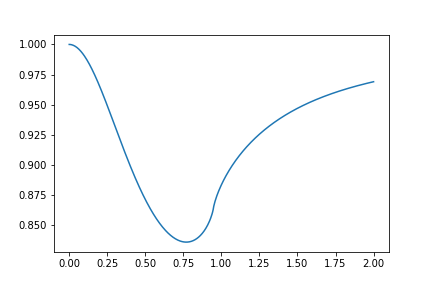
\includegraphics[width=0.7\linewidth]{2_site_ergo_theo}
	\caption{2 Site Max-Ergotropy}
	\label{fig:2siteergotheo}
\end{figure}
\begin{figure}[h]
	\centering
	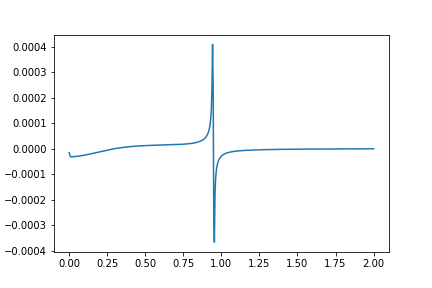
\includegraphics[width=0.7\linewidth]{2_site_ergo_theo_secdev}
	\caption{Second derivative 2 site Max-Ergotropy}
	\label{fig:2siteergotheosecdev}
\end{figure}
%Devi portare a 0 l'energia mi sa
\newpage
\subsection{Two distant sites}
Let's try substituting $g_1$ with $g_d$ with d distance between sites.
Eigenvalues of the correlation matrix as in (PHYSICAL REVIEW A 78, 052302 2008)
\begin{equation}
	\nu_{\pm}=\sqrt{\left(\frac{g_{d}-g_{-d}}{2}\right)^{2}+g_{0}^{2}} \pm \left| \frac{g_{d}+g_{-d}}{2} \right|
\end{equation}
Eigenvalues of the density matrix:
\begin{equation}
	p_{\pm \pm } =(1 \pm \nu_-)(1 \pm \nu_+)/4
\end{equation}




\bibliographystyle{alpha}
\bibliography{bibanalitic}

\nocite{*}
\end{document}